\section{Related Works}
\label{ch:relate}
\epigraph{If I have seen further it is by standing on the shoulders of Giants.}{Isaac Newton}

% - 讨论 client-side 的 clickstream 为什么值得研究,比较服务端搜集的 clickstream 产生的明显变化是什么。
% - 讨论现有的 client-side clickstream 研究分别是针对什么方向的,他们的结论主要是什么,都有什么样的改进空间。
% - 以前的 clickstream 只有类别级的分配模型,通过人工设计某个特定网站的马尔科夫模型来学习用户在不同类别之间的跳转概率。但当变为客户端后,数据变得更加充分,用户在一段时间内可能不局限于某个特定的网站,同时可能被其他网站干扰。

The previous research relating to this thesis is highlighted in this chapter. 
These research are the existing approaches to clickstream behavior modeling, 
the evolution of information behavior theory regarding and how it adapts to 
our digital world, and the most relevant recent advances regarding sequence learning.

\subsection{Clickstream Behavior Modeling}

\subsubsection{Server-side Clickstream Models}

Clickstream behavior research can be traced back to the year when the word ``clickstream''
was invented. Early clickstream behavior research has studied the navigational behavior
of user \cite{mandese1995clickstreams, brodwin1995}.
These research conducted binary classifications of clickstream based on the degree of linearity.

Mobasher et al. have discovered the effective and scalable techniques \cite{Mobasher:2001:EPB:502932.502935} 
for web personalization by using association rules and built a recommendation system. 
Goldfrab has investigated \cite{goldfarb2002analyzing} the website choice behavior based on 
clickstream data and has suggested that clickstreams simulate company strategy changes.
Chatterjee et al. \cite{chatterjee2003modeling} where the first to conduct 
research on clickstream with regard to an actual commercial website, 
and they found implies that dynamic advertising
based on customer clickstream history influences the future clickstream of the customer
and increases interactions with dynamic advertisement.
More technically, Ting et al. have used common sequences to determine 
unexpected browsing behavior \cite{Ting:2005:UMF:1092358.1092469}
and used their findings to improve website design. 

The most recent research has evolved the approaches of clickstream modeling,
Wang et al.\cite{Wang:2016:UCC:2858036.2858107} have proposed an unsupervised approach 
to model clickstream without labeling.
Chi et al. have proposed an analysis framework \cite{chi2017towards} for the general understanding 
of online information behavior in a specific page. 
However, their framework only fits for server-side collected clickstreams instead of 
a real user clickstream.

Then, Wang et al. \cite{Wang:2017:CUB:3127338.3068332} have improved their unsupervised approach
and summarized more comprehensive reviews of the existing approaches, 
such as common subsequences of clickstreams and graph clustering based classification 
for clickstream behavior modeling that identifies spam and abuse for a specific website. 
Based on Poisson process, Park et al. have modeled and detected a behavior change 
among students while learning \cite{Park:2017:DCS:3027385.3027430} to
help improve their online learning experience. Amo et al. \cite{amo2018learning} have 
further visualized search-stream behavior that serves student clickstream data from a class, 
and Shimada et al. have proved \cite{Shimada:2018:OCD:3170358.3170412} that
online change detection while monitoring student behavior is possible based on a sliding window.

Zaloudek has conducted a review of review on the comparison \cite{mastersthesis} traditional method 
to model clickstream data, and proposed a principle component analysis-based method for 
the semi-supervised learning of clickstream data. 
However their approach does not work well for clustering task, and 
the best performance is obtained by a traditional multilayer perceptron algorithm.
Chandramohan and Ravindran have further investigated the neural approach to 
clickstream mining \cite{N:2018:NAB:3152494.3152505},
and verified that based on a server-side collected clickstream, a complex recurrent unit 
with an attention mechanism can capture whether a user
has the intent to buy a product.
Surprisingly, Gundala and Spezzano \cite{Gundala:2018:RDH:3184558.3191644} have used a Lasso
regression based on sophisticated feature engineering with an 
archived area under the curve score 0.769 for reader demand hyperlink prediction 
on a Wikipedia clickstream dataset.

\subsubsection{Client-side Clickstream Models}

Kammenhuber et al. have produced the first study
regarding a client-side clickstream \cite{Kammenhuber:2006:WSC:1177080.1177110}. 
They have proposed a finite-state Markov model that models user's search behavior on a level of
topic categories. Unfortunately, their dataset was collected from network package traffic,
they did not consider the time and actions that a user spends and made on each page.


% 关于 assistent 的研究
% @article{lieberman1995letizia,
%   title={Letizia: An agent that assists web browsing},
%   author={Lieberman, Henry and others},
%   journal={IJCAI (1)},
%   volume={1995},
%   pages={924--929},
%   year={1995}
% }

\begin{figure}[H]
    \centering
    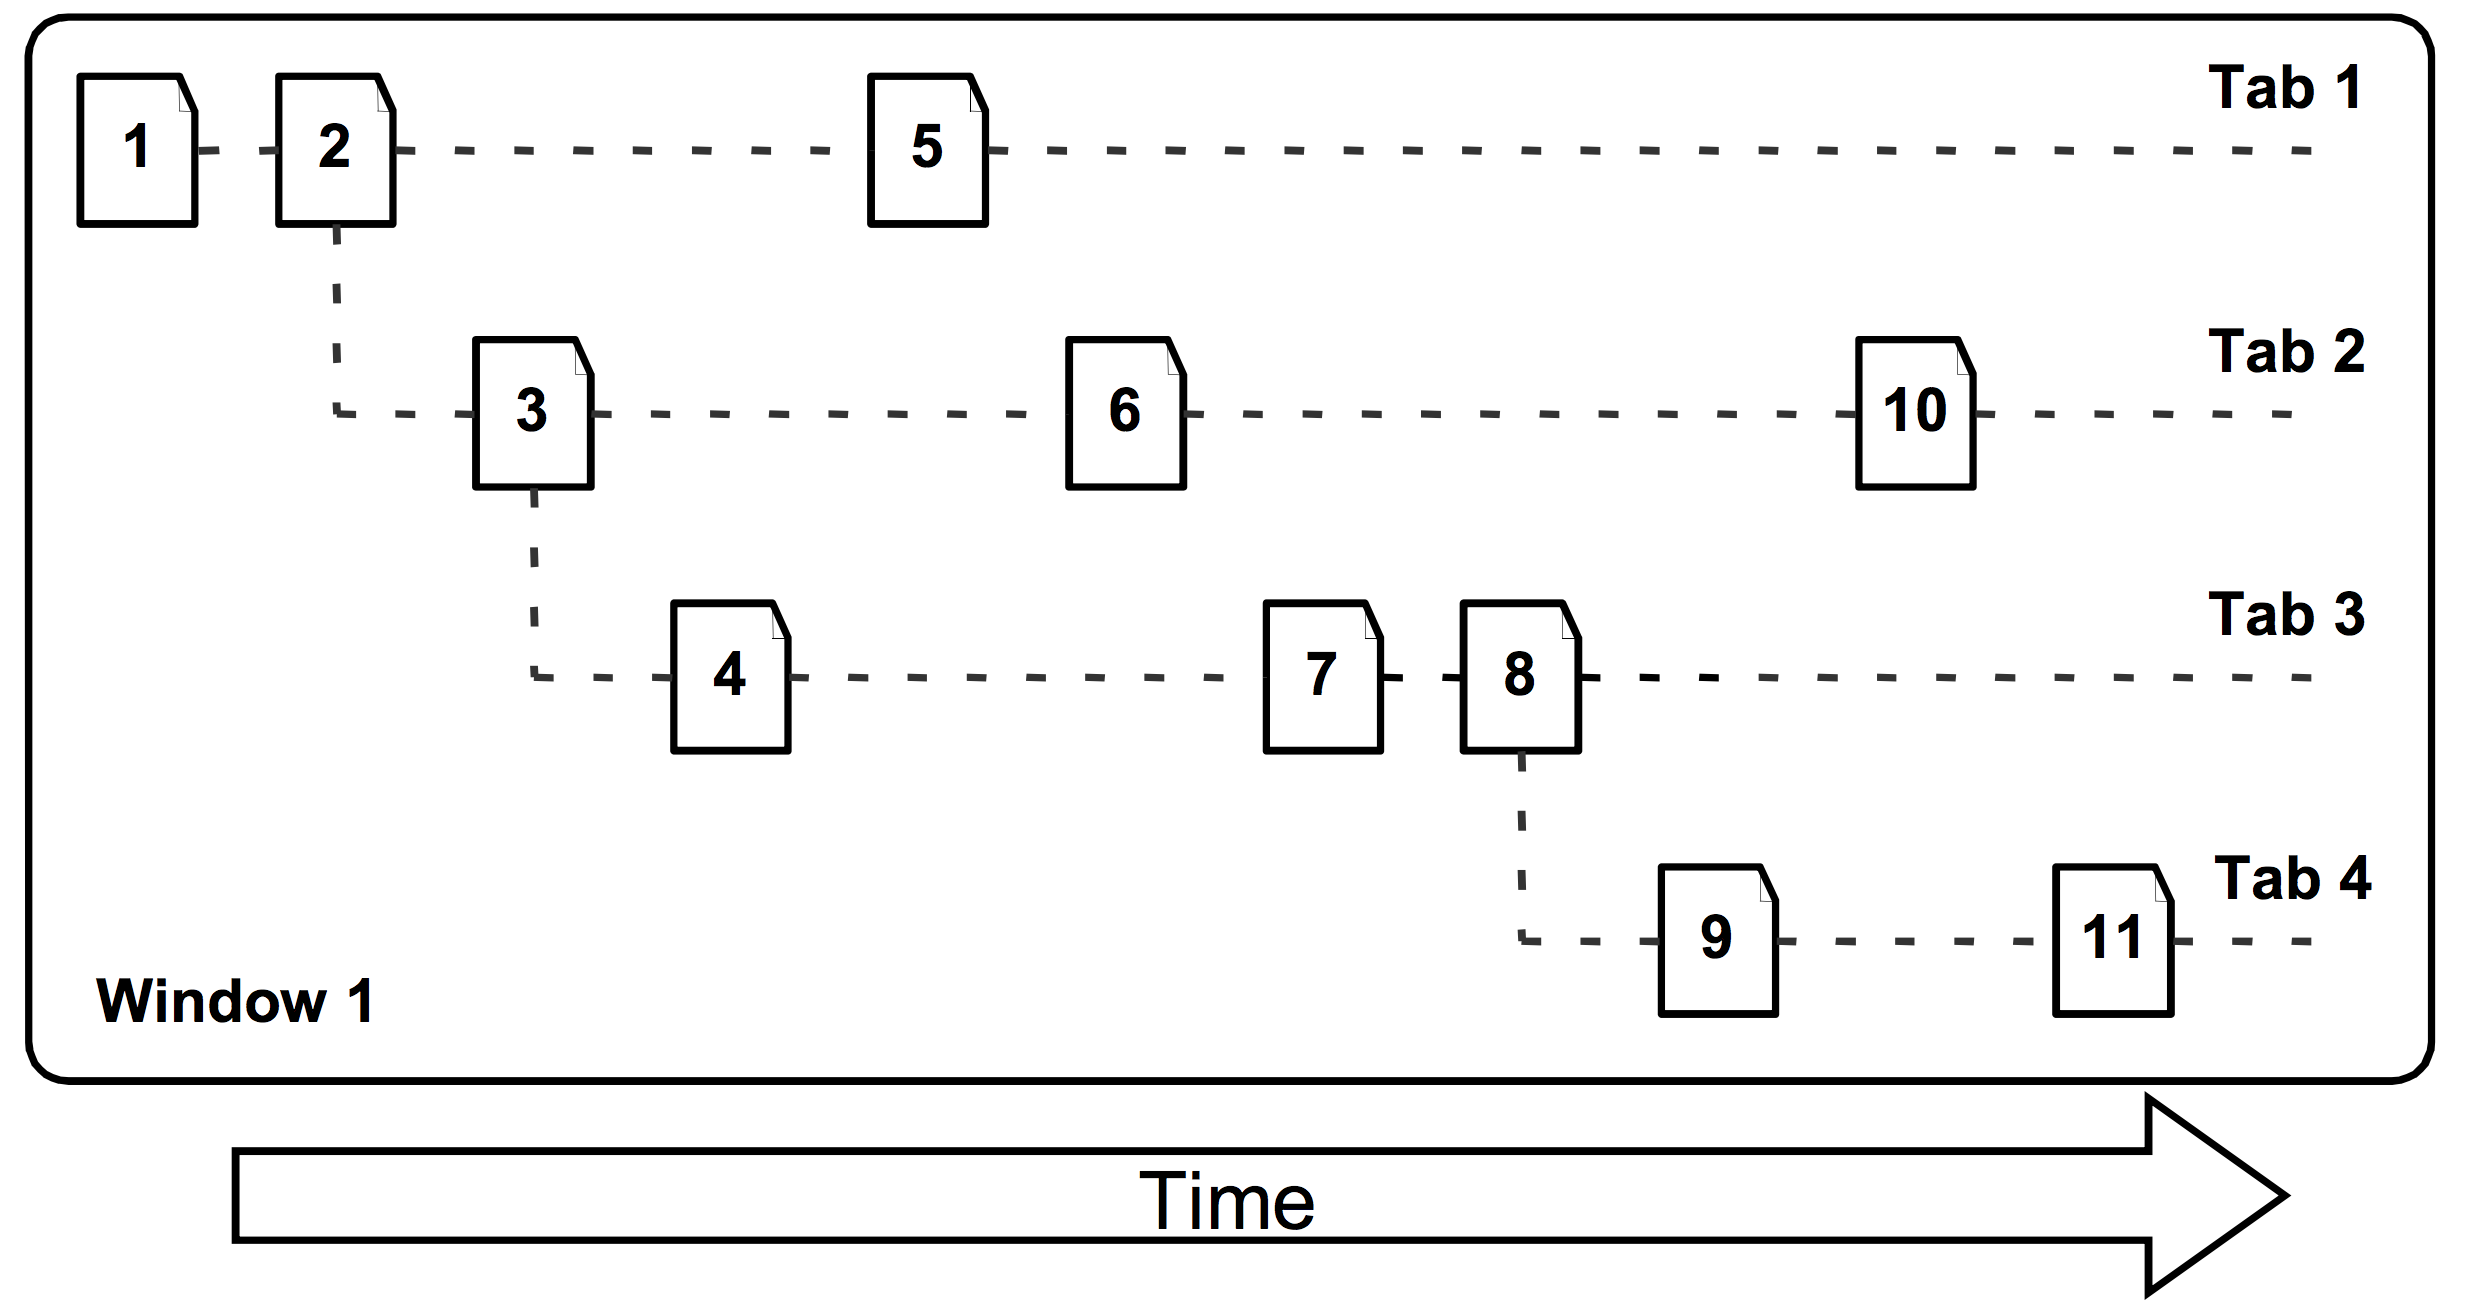
\includegraphics[width=0.55\textwidth]{figures/branching-and-backtracking}
    \caption{Parallel browsing behavior: branching phenomenon \cite{huang2010parallel}}
    \label{fig:backtrace}
\end{figure}

Liu et al. \cite{liu2010understanding} have studied specific user behavior on dwell time on web pages
and concluded that Weibull distribution is the most appropriate distribution for characterizing 
this behavior. 
Huang et al. \cite{huang2010parallel, huang2012no} have further 
noticed the behavior of branching parallel browsing and backtracking browsing
behavior on modern browsers, as depicted in Figure \ref{fig:backtrace}.
The authors have also presented a frequent analysis for the individual distribution of 
these two types of behavior.

The existing research regarding clickstream 
behavior modeling is either server-side modeling for an individual website or 
is individually modelized for client-side behaviors with limited information regarding clickstream,
which do not accurately represent the ground truths of user behavior. 
In any case, the existing approaches are based on self-constructed features, 
the property of Markov memoryless, and so on. Though the most recent
approaches use neural networks, their findings only applies to specific context.
From the point of view of user behavior, these previous approaches 
neither unambiguously justify the foundation of their model, 
nor enable a major performance improvement of their model.

In this thesis, the client-side chronologic URL sequences are serialized with combinations of all 
these individually studied phenomena, including the branching and backtracking browser 
feature. These chronologic URLs are used to understand and model the essential user 
behavior patterns while browsing on the web.


\subsection{Sequence to Sequence Learning}
\label{sec:seq-learn}

Sequence learning is a large scope of research and has been applied to many fields such as 
typical application machine translation in nature language processing. 

Recurrent neural network (RNN) have been described by Werbos \cite{werbos1990rnn} and 
Rumelhart et al. \cite{Rumelhart:1988:LRB:65669.104451}, the original RNN 
generalizes feedforward neural networks for sequence based data.

Given a sequence of input $(i_1, i_2, ..., i_T)$, the original RNN computes a
sequence of outputs $(o_1, o_2, ..., o_T)$ 
by iterating the activation function Equation \ref{eqn:bptt}:

\begin{align}
\label{eqn:bptt}
\begin{split}
    k_t &= \sigma \left( W_{hi}i_{t} + W_{hh}k_{t-1}\right) \\
    o_t &= W_{oh} k_t, t=1,2,...,T
\end{split}
\end{align}

where $\sigma(x) = \frac{1}{1+\exp\{-x\}}$ is a non-linear transformation function,
and $W_{oh}, W_{hh}, W_{hi}$ are weight parameters between output, hidden and input layers,
as shown in Figure \ref{fig:rnn}. 

\begin{figure}[H]
    \centering
    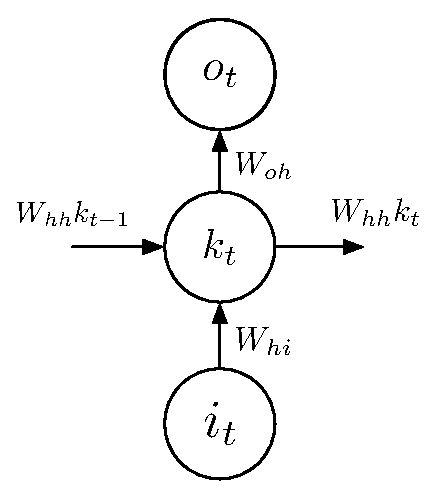
\includegraphics[width=0.30\textwidth]{figures/rnn}
    \caption{Vanilla recurrent unit: the original RNN uses linear weights 
    transformation and a $\sigma$ non-linear transformation between inputs and outputs 
    as a recurrent unit}
    \label{fig:rnn}
\end{figure}

The most widely used recurrent units in RNN are the
Long-Short-Term memory (LSTM) unit \cite{hochreiter1997lstm} 
or gated recurrent unit (GRU) \cite{DBLP:journals/corr/ChoMGBSB14}, These units provide a
performance than is significantly superior to traditional hidden Markov models 
in machine translation\cite{DBLP:journals/corr/abs-1901-01122}.

The LSTM unit has a context cell and three regulators: input gate, 
output gate and forget gate.
The context cell maintains dependencies between inputs of the unit as a form of long term memory. 
The input gate takes the historical hidden state as well as the current input and controls 
the input value to the recurrent unit. The output gate is responsible for the control of output activations. 
The forget gate resets and decides retaining values of the recurrent unit as a form of short-term memory.
Similarly, the GRU simplifies the structure of the LSTM into an update gate and a reset gate.

On the other hand, the vanilla RNN transfers and maps a sequence to another sequence if 
the inputs and the outputs are aligned with equal length. 
Apparently, the major constraint of the vanilla RNN
is that the model cannot address a problem if the inputs and outputs are provided 
in different lengths with complicated and non-monotonic relationships.

Stutskever et al. \cite{DBLP:journals/corr/SutskeverVL14} have presented a general end-to-end approach
to sequence learning models in machine translation that estimates the conditional probability of 
$p(o_1, o_2, ..., o_{T'} | i_1, i_2, ..., i_T)$ where $(i_1, i_2, ..., i_T)$ is an input sequence,
$(o_1, o_2, ..., o_{T'})$ is a corresponding output sequence, and $T$ does not have to equal with $T'$.

In machine translation, a series of words are considered to be a sequence of
vectors, and neural network-based models are considered to be representative of 
the learning of nature languages.
The initial vectors of word were one-hot encoded vectors and received updates over the training and learning.

The recent advances of representation learning uses a distributed representation 
of the word2vec model \cite{DBLP:journals/corr/abs-1301-3781}, which achieves better 
performance in natural language processing. The word2vec model introduced the 
continuous bag-of-word model and the skip-gram model as efficient methods for learning the high-quality
vector representation of words. The bag-of-word model is faster and the skip-gram model is slower 
but achieves better performance for infrequent words.

\subsection{Theory of Information Behavior on the Web}
\label{sec:info-seek}

The thesis relates to information behavior theory because it supports the foundation of our
user study. This subsection discusses how the theory was concluded and 
how the principles of the theory that sustain the thesis.

Information behavior research encompasses intentional information seeking and 
unintentional information encounters. The roots to information behavior 
theory relates to information needs and uses \cite{doi:10.1002/aris.2009.1440430114} 
that arose in the 1960s.

However, the concept of information seeking behavior, was coined in the late 1981s 
by Thomas Wilson \cite{wilson1981user}. He tries to formalize the process or 
activities of a conscious effort regarding information needs 
and uses. Figure \ref{fig:wilson-info-seek} illustrates the model of information behavior 
that was proposed.

\begin{figure}
    \centering
    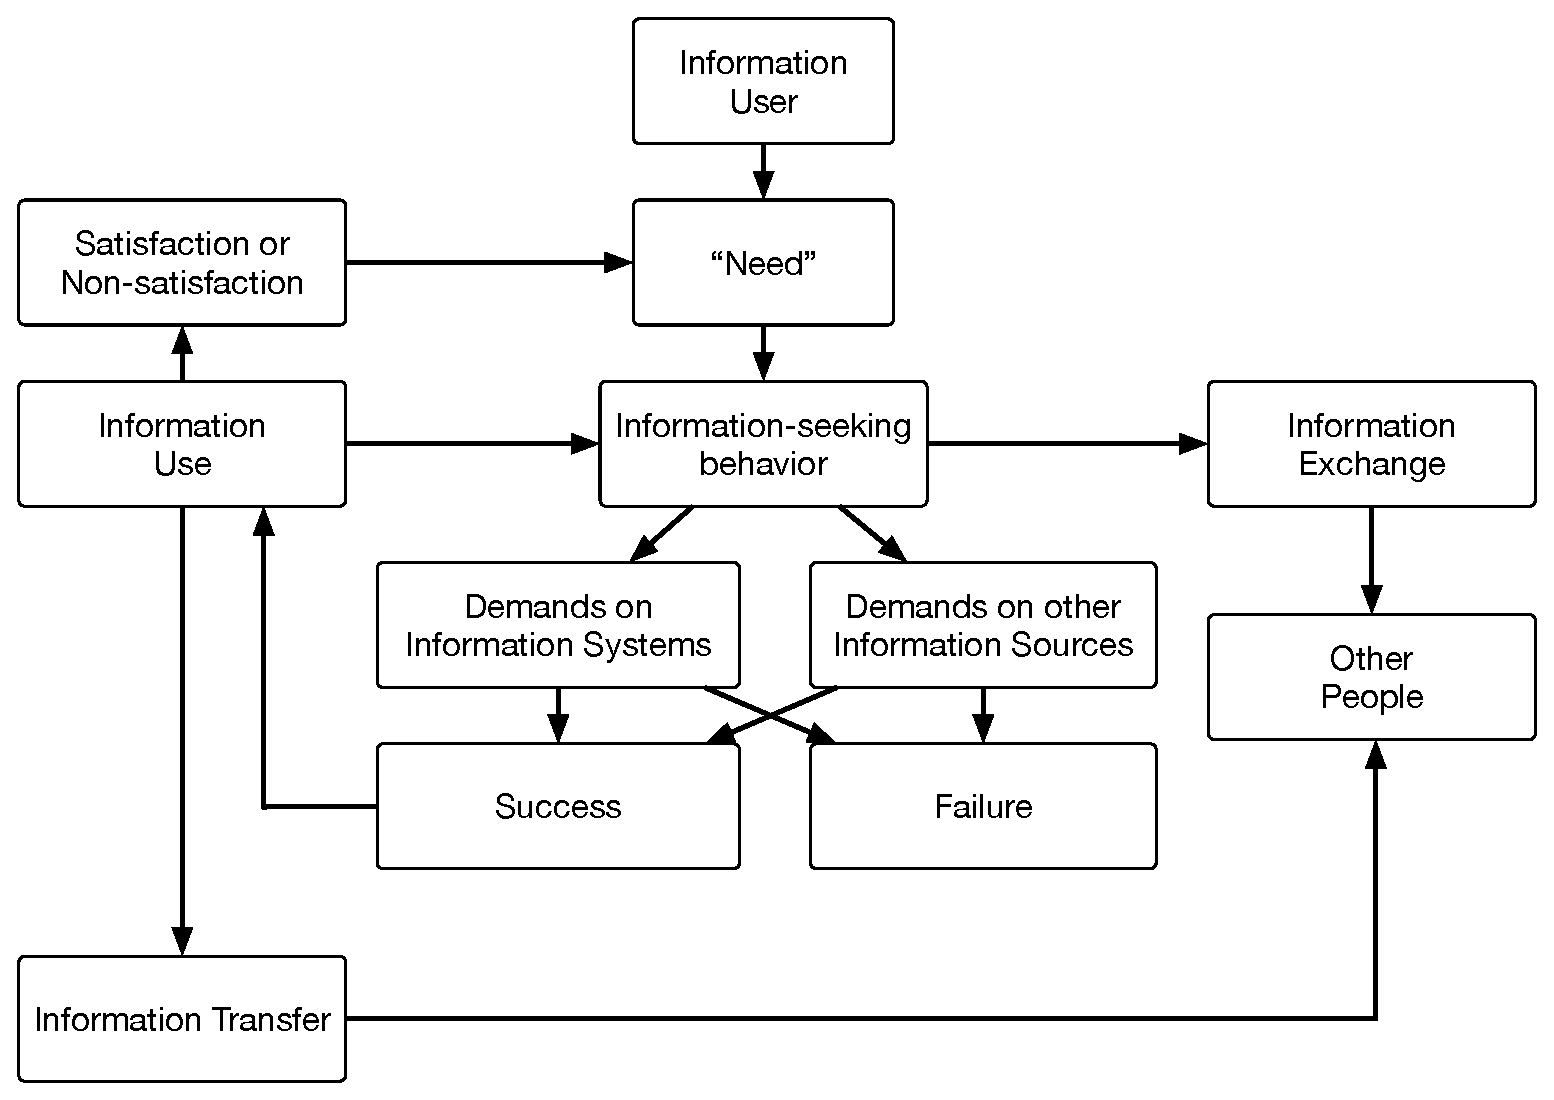
\includegraphics[width=0.7\textwidth]{figures/wilson-info-behavior}
    \caption{Wilson's information seeking behavior model \cite{wilson1981user}}
    \label{fig:wilson-info-seek}
\end{figure}

Wilson's model has been used for many years since its inception, and has been revised 
and adapted to our digital world because the digital systems learn user preferences and 
change \cite{giannini1998receiving} the way we receive information.

David Ellis has described a detailed group of activities for information seeking behavior \cite{ellis1989behavioural}
and applied it to the industrial as well as physical and social science \cite{ellis1993comparison} 
environments \cite{ellis1997modelling}.
His analysis was based on grounded theory approach \cite{aceto1994grounded} and semi-structured interviews. 

Choo et al. adapts Ellis' Model and discussed \cite{choo1999information}
the information seeking behavior on the web through different activities other than 
a single process. The activities are:
\textbf{\emph{starting, chaining, browsing, differentiating, monitoring, and extracting}}.

``\emph{Starting}'' on the web indicates that a user identifies websites or pages
that contain the information regarding their interests.
``\emph{Chaining}'' indicates that a user follows the starting page to other related pages.
``\emph{Browsing}'' represents the activity that a user engages in when they skim on the web
and quickly view the top-level information. 
``\emph{differentiating}'' describes how a user on the web selects useful pages 
and choose differentiated targets.
``\emph{Monitoring}'' activity is used for receiving updates on the sites or for revisiting
the previously visited pages. Finally, ``\emph{extracting}'' refers to a user
systematically extracting information from an interested page or website while browsing.

By applying these activities, Choo et al. \cite{choo1999information} 
have concluded that the general user behaviors 
on the web are undirected viewing, conditioned viewing, informal search and formal search.
Johnson has described further \cite{johnson2017patterns} for seven detailed behaviors 
patterns on the web but did not provide a working study that verified or proved their formation.

Although Wilson's model and Ellis' model are revised in recent works, these improvements
are more generic and are too complex for describing user information behavior on the web,
which cannot adapts to the experiment design (discuss detailly in Chapter \ref{ch:exp}
and Section \ref{sec:decision}).
This thesis uses an antecedent of Wilson's framework \cite{wilson1997information} and 
Ellis' model \cite{ellis1997modelling} to formalize and justify the lab study 
in Chapter \ref{ch:exp}. This experiment form the foundation of this work.

\cleardoublepage